\documentclass[11pt,letterpaper]{article}
\usepackage[utf8]{inputenc}
\usepackage{amsmath}
\usepackage{amsfonts}
\usepackage{amssymb}
\usepackage{fullpage}
\usepackage{hyphenat}
\usepackage{amsthm}
\usepackage{algorithm}
\usepackage{algorithmic}

\usepackage{tikz}
\usetikzlibrary{arrows}
\usetikzlibrary{shapes.geometric}

%\newcommand{\LP}{\textsc{link placement}}
%\newcommand{\HS}{\textsc{hitting set}}
\newcommand{\LP}{LINK PLACEMENT}
\newcommand{\HS}{HITTING SET}
\newcommand{\reals}{\mathbb{R}}

\newtheorem{lemma}{Lemma}

\begin{document}
\title{The Link Placement Problem}
\author{Bob West}
\maketitle


\section{Problem statement}

We formulate the problem of adding the optimal set of hyperlinks to a website, given a limited budget of links that may be added.
Limiting the number of new links may be important in practice, since links typically need to be added, or at least checked, by a human website administrator, which is time-consuming and costly, so we want to keep the load on the human low while still producing a good ensemble of links.

In the link placement problem we are given
\begin{enumerate}
\item a website represented as a hyperlink graph $G=(V,E)$ and
\item a set $P \subseteq V^*$ of navigation paths over this network
\end{enumerate}
and are asked for the $K$ best previously non-existent links $E' \subseteq V^2 \setminus E$ to be added to $G$.

Here, `best' can be defined according to a variety of objective functions.
We describe two in the next section.


\section{Objective functions}

\subsection{Maximizing the expected number of clicks on new links}

The first objective we consider captures the expected number of clicks received cumulatively by all newly added links.
This is a natural criterion, since it leads to a set of new links that will be used heavily and will therefore facilitate navigation.

In this setup, we imagine for each path $p=(p_1,\dots,p_n)$ that the user revisits the path step by step, and for each triple $(p_i,p_{i+1},p_{i+2})$ along the path for which $(p_i,p_{i+2}) \in E'$, the user has the option to choose the shortcut $(p_i,p_{i+2})$; i.e., in these cases the user may choose to skip over $p_{i+1}$.

We assume that, for each node triple $(s,m,t)$ with $(s,t) \in E'$, there is a fixed probability $q(s,m,t)$ with which the user will choose the shortcut $(s,t)$ over the full triple $(s,m,t)$.
This way, we can compute the probability of being chosen for each shortcut link along each path.
We emphasize that in this setup only single nodes can be skipped along a path, i.e., only forward\hyp triangle\hyp closing operations are allowed in $G$.

Consider a path $p=(p_1,\dots,p_n)$ and let $f^p_i$ be the probability that the (old) link $(p_i,p_{i+1})$ is clicked on path $p$, and $g^p_i$ the probability that the (new) link $(p_i,p_{i+2})$ is clicked.
We define $x(s,t)$ as a binary variable indicating whether $(s,t) \in E'$, i.e., whether $(s,t)$ is chosen in the solution.
Then the above path\hyp specific probabilities $f^p_i$ and $g^p_i$ are defined recursively as follows:

\begin{eqnarray}
\begin{array}{llll}
f^p_i &=& \left(f^p_{i-1} + g^p_{i-2}\right) \, (1 - x(p_i,p_{i+2}) \, q(p_i,p_{i+1},p_{i+2})) & \mbox{for $i=1,\dots,n-2$} \\
g^p_i &=& \left(f^p_{i-1} + g^p_{i-2}\right) \, x(p_i,p_{i+2}) \, q(p_i,p_{i+1},p_{i+2}) & \mbox{for $i=1,\dots,n-2$} \\
f^p_{i} &=& f^p_{i-1} + g^p_{i-2} & \mbox{for $i=n-1,n$} \\
f^p_0 &=& 1 & \\
g^p_{-1} &=& g^p_0 \;\;=\;\; g^p_{n-1} \;\;=\;\; g^p_n \;\;=\;\; 0 &
\end{array}
\label{eqn:f_and_g}
\end{eqnarray}

\begin{figure}
 \hspace*{-1.5cm}
 \centering
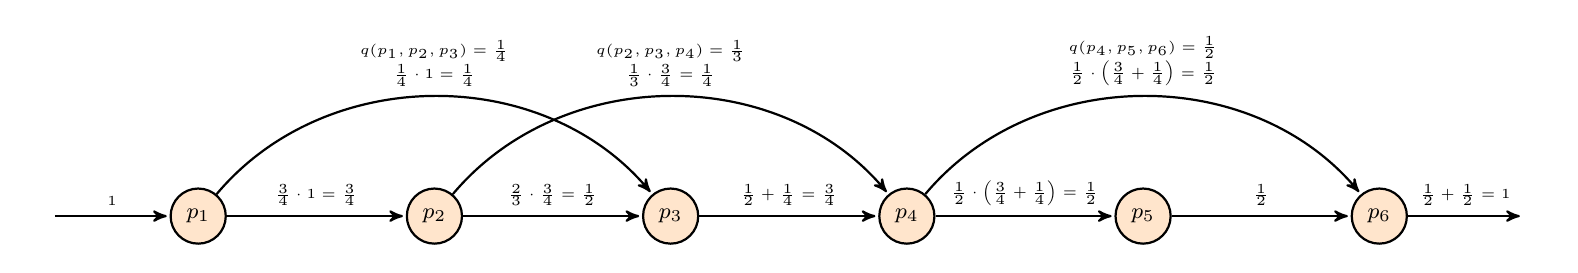
\begin{tikzpicture}[->,>=stealth',shorten >=1pt,auto,node distance=3cm,thick]

  \tikzstyle{p}=[circle,fill=orange!20,draw,font=\footnotesize,inner sep=0pt,minimum size=7mm]
  \tikzstyle{plain}=[circle,fill=white,font=\footnotesize]

  \node[plain] (p0) {};
  \node[p] (p1) [right of=p0, node distance=2cm] {$p_1$};
  \node[p] (p2) [right of=p1, node distance=3cm] {$p_2$};
  \node[p] (p3) [right of=p2, node distance=3cm] {$p_3$};
  \node[p] (p4) [right of=p3, node distance=3cm] {$p_4$};
  \node[p] (p5) [right of=p4, node distance=3cm] {$p_5$};
  \node[p] (p6) [right of=p5, node distance=3cm] {$p_6$};
  \node[plain] (p7) [right of=p6, node distance=2cm] {};
  \path[every node/.style={font=\tiny}]
    (p0) edge node {$1$} (p1)
    (p1) edge node {$\frac{3}{4}\cdot 1=\frac{3}{4}$} (p2)
    (p2) edge node {$\frac{2}{3}\cdot\frac{3}{4}=\frac{1}{2}$} (p3)
    (p3) edge node {$\frac{1}{2}+\frac{1}{4}=\frac{3}{4}$} (p4)
    (p4) edge node {$\frac{1}{2}\cdot\left(\frac{3}{4}+\frac{1}{4}\right)=\frac{1}{2}$} (p5)
    (p5) edge node {$\frac{1}{2}$} (p6)
    (p6) edge node {$\frac{1}{2}+\frac{1}{2}=1$} (p7);
  \path[every node/.style={font=\tiny}]
    (p1) edge [bend left=50] node[align=center] {$q(p_1,p_2,p_3)=\frac{1}{4}$\\$\frac{1}{4}\cdot 1=\frac{1}{4}$} (p3)
    (p2) edge [bend left=50] node[align=center] {$q(p_2,p_3,p_4)=\frac{1}{3}$\\$\frac{1}{3}\cdot\frac{3}{4}=\frac{1}{4}$} (p4)
    (p4) edge [bend left=50] node[align=center] {$q(p_4,p_5,p_6)=\frac{1}{2}$\\$\frac{1}{2}\cdot\left(\frac{3}{4}+\frac{1}{4}\right)=\frac{1}{2}$} (p6);

\end{tikzpicture}

\caption{Example showing how the probabilities $f^p_i$ and $g^p_i$ of being clicked are computed for a path $p$ based on the association prior click probabilities $q$ according to Eq.~\ref{eqn:f_and_g}. The straight arrows correspond to $f^p_i$'s, the bent arrows, to $g^p_i$'s.}
 \label{fig:shortcut_example}
\end{figure}

Note that this definition implies that, if $(p_i,p_{i+2}) \notin E'$, then $g^p_i=0$.

The above equations allow an interpretation in terms of network flow: one unit of flow is transmitted from $p_1$ to $p_n$, and the flow that enters each node must equal the flow that leaves it.
See Fig.~\ref{fig:shortcut_example} for an example.

The new links are not independent but interact with each other (Fig.~\ref{fig:shortcut_example}), so the flows over the new links depends on the entire set $E'$ of new shortcut links.
It is this interaction between links that makes the problem hard (in fact NP-hard, as we shall see).

Each newly introduced shortcut link $(s,t) \in E'$ may appear in several paths and has a probability of being clicked on each of these paths.
By summing these probabilities for fixed $(s,t)$ across all paths, we obtain the number of clicks that shortcut is expected to receive.

So we can now phrase our optimization objective: given a budget of $K$ shortcut links that may be added, choose those shortcuts that would receive the maximum expected number of clicks.
More formally, we want to maximize
\begin{eqnarray}
\psi(E') &=& \sum_{p \in P} \psi_p(E') \\
&=& \sum_{p \in P} \sum_{i=1}^{|p|-2} g^p_i,
\end{eqnarray}
where $|p|$ is the number of nodes on path $p$.





\subsubsection*{Integer linear program}

Note that in the above flow constraints (Eq.~\ref{eqn:f_and_g}), there is multiplicative interaction between the $f$ and $g$, and the $x$, variables.

It is nevertheless possible to formulate our optimization problem using only linear constraints (note that the $q$ terms are constants, while the $f$, $g$, and $x$ terms are optimization variables):

\begin{equation}
\text{maximize } \sum_{p \in P} \sum_{i=1}^{|p|-2} g^p_i \;\;\; \text{ subject to}
\label{eqn:ILP_objective}
\end{equation}

\begin{equation}
\begin{array}{rlll}
f^p_i + g^p_i &=& f^p_{i-1} + g^p_{i-2} & \mbox{for $i=1,\dots,n$} \\
g^p_i &\leq& x(p_i, p_{i+2}) & \mbox{for $i=1,\dots,n-2$} \\
g^p_i &\leq& \left(f^p_{i-1} + g^p_{i-2}\right) q(p_i,p_{i+1},p_{i+2}) & \mbox{for $i=1,\dots,n-2$} \\
f^p_0 &=& 1 & \\
g^p_{-1} &=& g^p_0 \;\;=\;\; g^p_{n-1} \;\;=\;\; g^p_n \;\;=\;\; 0 & \\
\sum_{(s,t) \in V^2} x(s,t) &\leq& K &  \\
x(s,t) &=& 0 & \mbox{for $(s,t) \in E$} \\
x(s,t) &\in& \{0,1\} & \mbox{for $(s,t) \in V^2$} \\
\end{array}
\label{eqn:ILP_constraints}
\end{equation}

The problem is made hard by the integrality constraint $x(s,t) \in \{0,1\}$.




\subsection{Maximizing the expected number of paths with a click on a new link}

Our second objective function is more path- than link-centric.
It considers the expected number of paths in which at least one shortcut click is clicked.
Formally, the objective function is
\begin{eqnarray}
\phi(E')  &=& \sum_{p \in P} \phi_p(E') \\
          &=& \sum_{p \in P} \left( 1 - \prod_{i=1}^{|p|-2} \left( 1 - x(p_i,p_{i+2}) \, q(p_i,p_{i+1},p_{i+2}) \right) \right),
\end{eqnarray}
where $x(s,t)$ is again a binary variable indicating whether $(s,t)$ is part of the solution.

We use $\phi_p(E')$ to denote the value of the solution $E'$ when discarding all paths but $p$.
It captures the probability of at least one shortcut being clicked in path $p$.
The total value $\phi(E')$ is then obtained by summing over all path-wise values and captures the expected number of paths with at least one shortcut click.

In the previous objective $\psi$ we could only handle shortcuts skipping a single node, since it isn't clear how the flow would be distributed if several shortcuts were available from the same source.
In the case of $\phi$, on the other hand, handling long-range links skipping more than a single node (and thus handling potentially several shortcuts from the same source) is straightforward:
Since we start from the probability that {\em no} link is clicked (and then subtract it from one to get the probability that at least one link is clicked), we can simply multiply the probabilities of the single links not being clicked.
In other words, computing the probability of no flow is conceptually simpler than computing how the flow is divided up.




\section{NP-hardness}

Now we show that our problem is dang hard.
We start with the link-based objective $\psi$ and then show that the same reasoning can be used to prove that optimizing the path-based objective $\phi$ is NP-hard.


\subsection{Hardness of optimizing $\psi$}

We already saw that our problem can be formulated as an integer linear program.
Solving integer linear programs is in general NP-hard, and here we show that this is also true for our specific case.

We proceed by reducing \HS{}%
\footnote{Garey and Johnson: {\it Computers and Intractability,} 1979, Problem SP8, p.~222.}
to our problem of maximizing $\psi$.
But first we formally define the \LP{} and \HS{} problems.

\subsubsection{Definition of the \LP{} problem}

\begin{itemize}
\item {\bf Instance:} Directed graph $G=(V,E)$;
set of paths $P \subseteq V^*$;
positive integer $K$;
a shortcut probability for each node triple, i.e., a mapping $q : V^3 \rightarrow [0,1]$.
\item {\bf Question:} Given a budget of $K$ shortcut links $(s_1,t_1), \dots, (s_K,t_K)$, what is the maximum cumulative flow over the shortcuts across all paths, according to the model of Eq.~\ref{eqn:f_and_g}?
\end{itemize}

\subsubsection{Definition of the \HS{} problem}

\begin{itemize}
\item {\bf Instance:} Collection $C$ of subsets of a finite set $Z$, positive integer $L \leq |Z|$.
\item {\bf Question:} Is there a subset $Z' \subseteq Z$ with $|Z'| \leq L$ such that $Z'$ contains at least one element from each subset in $C$?
\end{itemize}

Importantly, the problem remains NP-complete even if $|c| \leq 2$ for all $c \in C$.

\subsubsection{Reduction}

We need to reduce a \HS{} instance $(C,Z,L)$ to a \LP{} instance $(V,E,P,q,K)$.
We assume w.l.o.g.\ that each $c \in C$ contains at most two elements.
(As stated above, \HS{} remains NP-complete even in this special case.)

First, we construct the hyperlink network $G=(V,E)$.
For each $z_i \in Z$ we include three nodes $s_i,m_i,t_i$ in the hyperlink network:
\begin{equation}
V=\bigcup_{i=1}^{|Z|} \{s_i, m_i, t_i\}.
\end{equation}

Next, we construct the set $P$ of paths over these nodes. We construct one path per subset $c \in C$:
if $c=\{z_j,z_k\}$, we add the path $(s_j,s_k,t_j,t_k)$, and if $c=\{z_j\}$, we add the path $(s_j,m_j,t_j)$:
\begin{equation}
P = \bigcup_{\{z_j,z_k\} \in C} \{(s_j, s_k, t_j, t_k)\} \cup \bigcup_{\{z_j\} \in C} \{(s_j, m_j, t_j)\}.
\end{equation}

The edge set $E$ of $G$ is now simply defined as the set of edges induced by $P$:
\begin{equation}
E = \bigcup_{\{z_j,z_k\} \in C} \{(s_j,s_k), (s_k,t_j), (t_j,t_k)\} \cup \bigcup_{\{z_j\} \in C} \{(s_j,m_j), (m_j,t_j)\}.
\end{equation}

The probability of taking a shortcut, in the case it exists, is set to 1 for all shortcut candidates:
\begin{equation}
q(s,m,t) = 1, \;\;\;\; \mbox{for all $(s,m,t) \in V^3$}.
\end{equation}

And finally,
\begin{equation}
K=L.
\end{equation}


\begin{figure}
 \centering
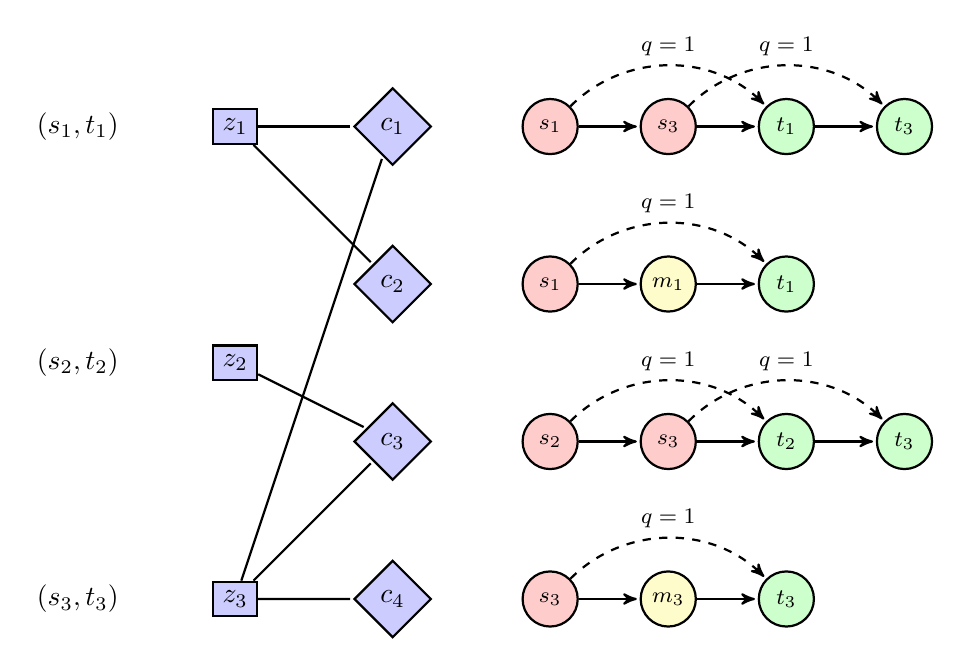
\begin{tikzpicture}[-,>=stealth',shorten >=1pt,auto,node distance=3cm,thick]

  \tikzstyle{plain}=[]
  \tikzstyle{elem}=[rectangle,fill=blue!20,draw]
  \tikzstyle{subset}=[diamond,fill=blue!20,draw]
  \tikzstyle{s}=[circle,fill=red!20,draw,font=\footnotesize,inner sep=0pt,minimum size=7mm]
  \tikzstyle{m}=[circle,fill=yellow!20,draw,font=\footnotesize,inner sep=0pt,minimum size=7mm]
  \tikzstyle{t}=[circle,fill=green!20,draw,font=\footnotesize,inner sep=0pt,minimum size=7mm]

  \node[elem] (u1) {$z_1$};
  \node[elem] (u2) [below of=u1] {$z_2$};
  \node[elem] (u3) [below of=u2] {$z_3$};

  \node[plain] (st1) [left of=u1, node distance=2cm] {$(s_1,t_1)$};
  \node[plain] (st2) [below of=st1] {$(s_2,t_2)$};
  \node[plain] (st3) [below of=st2] {$(s_3,t_3)$};

  \node[subset] (c1) [right of=u1, node distance=2cm] {$c_1$};
  \node[subset] (c2) [below of=c1, node distance=2cm] {$c_2$};
  \node[subset] (c3) [below of=c2, node distance=2cm] {$c_3$};
  \node[subset] (c4) [below of=c3, node distance=2cm] {$c_4$};

  \path[every node/.style={font=\small}]
    (u1) edge (c1)
    (u3) edge (c1)
    (u1) edge (c1)
    (u1) edge (c2)
    (u2) edge (c3)
    (u3) edge (c3)
    (u3) edge (c4);

  \node[s] (p11) [right of=c1, node distance=2cm] {$s_1$};
  \node[s] (p12) [right of=p11, node distance=1.5cm] {$s_3$};
  \node[t] (p13) [right of=p12, node distance=1.5cm] {$t_1$};
  \node[t] (p14) [right of=p13, node distance=1.5cm] {$t_3$};
  \path[->]
    (p11) edge (p12)
    (p12) edge (p13)
    (p13) edge (p14);
  \path[->,every node/.style={font=\footnotesize}]
    (p11) edge [bend left=45, dashed] node {$q=1$} (p13)
    (p12) edge [bend left=45, dashed] node {$q=1$} (p14);

  \node[s] (p21) [right of=c2, node distance=2cm] {$s_1$};
  \node[m] (p22) [right of=p21, node distance=1.5cm] {$m_1$};
  \node[t] (p23) [right of=p22, node distance=1.5cm] {$t_1$};
  \path[->]
    (p21) edge (p22)
    (p22) edge (p23);
  \path[->,every node/.style={font=\footnotesize}]
    (p21) edge [bend left=45, dashed] node {$q=1$} (p23);

  \node[s] (p31) [right of=c3, node distance=2cm] {$s_2$};
  \node[s] (p32) [right of=p31, node distance=1.5cm] {$s_3$};
  \node[t] (p33) [right of=p32, node distance=1.5cm] {$t_2$};
  \node[t] (p34) [right of=p33, node distance=1.5cm] {$t_3$};
  \path[->]
    (p31) edge (p32)
    (p32) edge (p33)
    (p33) edge (p34);
  \path[->,every node/.style={font=\footnotesize}]
    (p31) edge [bend left=45, dashed] node {$q=1$} (p33)
    (p32) edge [bend left=45, dashed] node {$q=1$} (p34);

  \node[s] (p41) [right of=c4, node distance=2cm] {$s_3$};
  \node[m] (p42) [right of=p41, node distance=1.5cm] {$m_3$};
  \node[t] (p43) [right of=p42, node distance=1.5cm] {$t_3$};
  \path[->]
    (p41) edge (p42)
    (p42) edge (p43);
  \path[->,every node/.style={font=\footnotesize}]
    (p41) edge [bend left=45, dashed] node {$q=1$} (p43);

\end{tikzpicture}

\caption{The reduction from \HS{} to \LP{}.
{\bf Blue:} the \HS{} instance.
{\bf Red/yellow/green:} the paths constructed for the \LP{} instance.
}
 \label{fig:reduction}
\end{figure}

The reduction is schematized in Fig.~\ref{fig:reduction}.
We now prove that by optimizing the \LP{} instance we could decide the \HS{} instance.
Therefore, \LP{} is at least as hard as \HS{}, which makes \LP{} NP-hard, since \HS{} is NP-complete.

In particular, we show that in the \HS{} instance we can hit all $|C|$ subsets with at most $K$ elements from $Z$ if and only if in the \LP{} instance the maximum shortcut flow that can be achieved by adding at most $K$ new shortcut edges is $|C|$.
The \HS{} instance could then be decided by computing the maximum for the \LP{} instance and checking if that maximum equals $|C|$.

The above equivalence can easily be verified in the sketch from Fig.~\ref{fig:reduction}.
Choosing $z_i$ in the \HS{} instance corresponds to introducing the shortcut $(s_i,t_i)$ in the \LP{} instance, and hitting subset $c$ corresponds to having at least one shortcut link available in the path corresponding to $c$.
Further, given the interleaving way in which the paths are constructed, and since all shortcut probabilities are 1, exactly one shortcut will be traversed in every path with at least one shortcut.
Hence, if all $|C|$ subsets can be hit in \HS{}, then the maximum shortcut flow is $|C|$ in \LP{}, and {\it vice versa}.


\subsection{Hardness of optimizing $\phi$}

Given the above proof, it is not hard to see that optimzing $\phi$ is NP-hard as well.
The paths in the \LP{} instance were constructed such that, whenever a path contains at least one shortcut, exactly one shortcut is clicked.
Therefore the number of shortcut clicks in a path equals the probability that at least one shortcut is clicked:
if the path contains a shortcut, both are 1, otherwise both are 0.

Hence, $\psi=\phi$ in the special case of paths as constructed in our reduction, and it follows that optimizing $\phi$ is NP-hard as well.



\section{Approximate solution via submodularity}

Not all NP-hard problems are equally hard. Some allow efficient approximations, others don't.
While both $\psi$ and $\phi$ are NP-hard, we'll now show that $\phi$ has a property that allows for high-quality approximation via a greedy algorithm, while $\psi$ doesn't have this property.

This property is submodularity.
Monotone submodular functions may be maximized approximately with a $(1-1/e)$-approximation guarantee ($1-1/e \approx 63\%$) via greedy marginal\hyp gain optimization.

\subsection{Non-submodularity of $\psi$}

First, we consider the case of $\psi$.
Recall that $\psi : 2^{V \times V} \rightarrow \reals$ computes the cumulative expected flow over all shortcut edges.
The counterexample of Fig.~\ref{fig:counterexample} shows that $\psi$ is not submodular.

\subsection{Submodularity of $\phi$}

\begin{figure}
 \centering
\begin{tikzpicture}[->,>=stealth',shorten >=1pt,auto,node distance=3cm,thick]

  \tikzstyle{p}=[circle,fill=orange!20,draw,font=\footnotesize,inner sep=0pt,minimum size=7mm]
  \tikzstyle{plain}=[circle,fill=white,font=\footnotesize]

  \node[p] (p1) [right of=p0, node distance=2cm] {$p_1$};
  \node[p] (p2) [right of=p1, node distance=3cm] {$p_2$};
  \node[p] (p3) [right of=p2, node distance=3cm] {$p_3$};
  \node[p] (p4) [right of=p3, node distance=3cm] {$p_4$};
  \node[p] (p5) [right of=p4, node distance=3cm] {$p_5$};
  \path
    (p1) edge (p2)
    (p2) edge (p3)
    (p3) edge (p4)
    (p4) edge (p5);
  \path
    (p1) edge [bend left=50] node[align=center] {$x$} (p3)
    (p2) edge [bend left=50] node[align=center] {$y$} (p4)
    (p3) edge [bend left=50, dashed] node[align=center] {$z$} (p5);

\end{tikzpicture}

\caption{Example showing that the objective $\psi$ is not submodular. If the $q$-values for all edges are defined as 1 then $\psi(\{x,y,z\}) - \psi(\{x,y\}) = 2-1 > 1-1 = \psi(\{y,z\}) - \psi(\{y\})$.}
 \label{fig:counterexample}
\end{figure}

Our second objective $\phi$, however, is monotone submodular, as shown by the following lemma.

\begin{lemma}
\label{thm:monotonicity}
The function $\phi$ is monotone increasing (i.e., $\phi(B) \geq \phi(A)$ if $A \subseteq B$) and submodular (i.e., $\phi(B \cup \{y\}) - \phi(B) \leq \phi(A \cup \{y\}) - \phi(A)$ if $A \subseteq B$).
\end{lemma}

\begin{proof}[Proof]
Without loss of generality, we need to consider only the case where $B$ is one element larger than $A$, i.e., $B = A \cup \{z\}$; the lemma will then follow by transitivity. Further, we may consider only the path\hyp specific function $\phi_p$; the lemma will then also hold for $\phi$, since the sum of submodular functions is also a submodular function.

Monotonicity is easy to see: Certainly, the probability of taking at least one link doesn't decrease if there are more links available. More formally, let $I_A$ and $I_B$ be the sets of indices at which the links from $A$ and $B$, respectively, start in $p$; and $k$, the index at which $z$ starts (if $z$ doesn't appear in $p$, $\phi_p(B)=\phi_p(A)$ trivially).
Also define $q^p_i = q(p_i,p_{i+1},p_{i+2})$.
Then,
\begin{eqnarray}
\phi_p(B)  &=& 1 - \prod_{i \in I_B} \left( 1 - q^p_i \right) \\
                      &=& 1 - (1 - q^p_k) \prod_{i \in I_A} \left( 1 - q^p_i \right) \\
                      &\geq& 1 - \prod_{i \in I_A} \left( 1 - q^p_i \right) \\
                      &=& \phi_p(A).
\end{eqnarray}

Submodularity is also straightforward. Let $k$ again be the index where $z$ starts, and $j$, the index where $y$ starts (if $y$ and $z$ don't both appear in $p$, then $\phi_p(B \cup \{y\}) - \phi_p(B) = \phi_p(A \cup \{y\}) - \phi_p(A)$). Then,
\begin{eqnarray}
\phi_p(B \cup \{y\}) - \phi_p(B) 
  &=& \left(1 - (1 - q^p_j) \prod_{i \in I_B} \left( 1 - q^p_i \right)\right)
    - \left(1 - \prod_{i \in I_B} \left( 1 - q^p_i \right)\right) \\
  &=& q^p_j \prod_{i \in I_B} \left( 1 - q^p_i \right) \\
  &=& (1 - q^p_k) \, q^p_j \prod_{i \in I_A} \left( 1 - q^p_i \right) \\
  &\leq& q^p_j \prod_{i \in I_A} \left( 1 - q^p_i \right) \\
  &=& \left(1 - (1 - q^p_j) \prod_{i \in I_A} \left( 1 - q^p_i \right)\right)
    - \left(1 - \prod_{i \in I_A} \left( 1 - q^p_i \right)\right) \\
  &=& \phi_p(A \cup \{y\}) - \phi_p(A).
\end{eqnarray}
\end{proof}





\subsection{Greedy algorithm}

(This section contains only jotted-down notes.)

- A greedy algorithm has a $(1-1/e)$-approximation guarantee for submodular objective functions.

- Here we assume $q$ is a function of $s$ and $t$ only

- Lazy: when shortcut $y$ is chosen and unpolluted, all links that co-occur with $y$ in any path must be marked polluted

- When $y$ is chosen but polluted, recompute its marginal gain: For each path $p$ containing $y$, increase the marginal gain of $y$ by 
$$\phi_p(A \cup \{y\}) - \phi_p(A)
\;\;\;=\;\;\; q^p_j \prod_{i \in I_A} \left( 1 - q^p_i \right),$$
where $A$ is the current set of shortcuts, and $j$, the index of $y$ in $p$.

\begin{algorithm}[t]
\caption{Greedy link placement}
% [1] adds line numbering:
\begin{algorithmic}[1]
\label{alg:greedy}
\INPUT hyperlink graph $G=(V,E)$; set $P \subseteq V^*$ of navigation paths; click probabilities $q$; number $K$ of links to be added to $G$
\OUTPUT set $E' \subseteq V^2 \setminus E$ of $K$ links to be added to $G$
\STATE $E' \leftarrow \{\}$ \hspace*{1mm}// \textit{the solution}
\STATE $Q \leftarrow \mathtt{PriorityQueue()}$ \hspace*{1mm}// \textit{the remaining link candidates}
\STATE $L \leftarrow \mathtt{HashTable()}$ \hspace*{1mm}// \textit{maps a source--target pair to the corresponding link-candidate object}
\STATE $M \leftarrow \mathtt{HashTable()}$ \hspace*{1mm}// \textit{maps a source--target pair to the set of paths in which it appears}
\STATE  // \textit{Store for each source--target pair in which paths it appears}
\FOR{all paths $p \in P$}
  \FOR{all link candidates $(s,t)$ appearing in $p$}
    \STATE $M[s,t] \leftarrow M[s,t] \cup \{p\}$ \hspace*{1mm}// \textit{Here we should impose a frequency threshold}
  \ENDFOR
\ENDFOR
\STATE  // \textit{Initialize all link canidates and build priority queue}
\FOR{all link candidates $(s,t) \in M.\mathtt{keys}$}
  \STATE $\ell \leftarrow \mathtt{LinkCandidate}(\mathtt{paths}=M[s,t], \mathtt{prob}=q(s,t), \mathtt{polluted}=\mathtt{false})$ %\hspace*{1mm}// \textit{last argument specifies that $\ell$ is unpolluted}
  \STATE $L[s,t] \leftarrow \ell$
  \STATE $Q[\ell] \leftarrow \mathtt{MarginalGain}(\ell, \{\})$
\ENDFOR
\STATE  // \textit{Construct the solution}
\FOR{$c = 1, \dots, K$}
  \WHILE{$\mathtt{true}$}
  	\STATE $\ell \leftarrow Q.\mathtt{poll()}$
    \IF{$\ell.\mathtt{polluted} = \mathtt{true}$}
      \STATE $Q[\ell] \leftarrow \mathtt{MarginalGain}(\ell, E')$
      \STATE $\ell.\mathtt{polluted} \leftarrow \mathtt{false}$
    \ELSE
      \FOR{$p \in \ell.\mathtt{paths}$}
        \FOR{all link candidates $(s,t)$ appearing in $p$}
          \STATE $L[s,t].\mathtt{polluted} \leftarrow \mathtt{true}$
        \ENDFOR
      \ENDFOR
      \STATE $E' \leftarrow E' \cup \{\ell\}$
      \STATE \textbf{break}
    \ENDIF
  \ENDWHILE
\ENDFOR
\end{algorithmic}
\end{algorithm}

\begin{algorithm}[t]
\caption{Marginal-gain computation: \texttt{MarginalGain}}
% [1] adds line numbering:
\begin{algorithmic}[1]
\label{alg:marginal_gain}
\INPUT link candidate $\ell$; current solution $E'$
\OUTPUT marginal gain of $\ell$ when added to the current solution $E'$
\STATE $m \leftarrow 0$
\FOR{$p \in \ell.\mathtt{paths}$}
  \STATE $j \leftarrow$ starting position of $\ell$ in $p$
  \STATE $I \leftarrow$ starting positions of the links from $E'$ in $p$
  \STATE $m \leftarrow m + q^p_j \prod_{i \in I} (1 - q^p_i)$
\ENDFOR
\STATE \textbf{return} $m$
\end{algorithmic}
\end{algorithm}


\section{TODO}

- In all of the above, we assumed that we have probabilities $q$ of a shortcut being taken if it existed.
In practice, we need to estimate these probabilities from data, which is itself a challenging problem.

- Plan: Identify all links that were added in February. For each link, derive features from the time before the link was added (such as our metrics inspired by frequent-item-set mining), in order to predict the probability with which the link will be clicked after the link was added.

- More formally, is $(s,t)$ is the link, the dependent variable is the number paths on which a direct click from $s$ to $t$ occurred, divided by the number of paths on which $s$ occurred before $t$.

- Work with Stanford CS and/or SimTk logs


\end{document}
